\documentclass[letter, 10pt]{article}
\usepackage[utf8]{inputenc}
\usepackage[latin1]{inputenc}
\usepackage[spanish]{babel}
\usepackage{amsfonts}
\usepackage{subcaption}
\usepackage{amsmath}
\usepackage{graphicx}
\usepackage{multirow}
\usepackage{longtable}
\usepackage{lscape}
\usepackage{url}
\usepackage{float}
\usepackage{listings}
\usepackage[top=3cm,bottom=3cm,left=3.5cm,right=3.5cm,footskip=1.5cm,headheight=1.5cm,headsep=.5cm,textheight=3cm]{geometry}


\begin{document}
\title{Inteligencia Artificial \\ \begin{Large}Informe Final: Milk Collection Problem with Blending solved with EA\end{Large}}
\author{[Branco Catalán]}
\date{\today}
\maketitle


%--------------------No borrar esta secci\'on--------------------------------%
\section*{Evaluaci\'on}

\begin{tabular}{ll}
Mejoras 1ra Entrega (10 \%): &  \underline{\hspace{2cm}}\\
C\'odigo Fuente (10 \%): &  \underline{\hspace{2cm}}\\
Representaci\'on (15 \%):  & \underline{\hspace{2cm}} \\
Descripci\'on del algoritmo (20 \%):  & \underline{\hspace{2cm}} \\
Experimentos (10 \%):  & \underline{\hspace{2cm}} \\
Resultados (10 \%):  & \underline{\hspace{2cm}} \\
Conclusiones (20 \%): &  \underline{\hspace{2cm}}\\
Bibliograf\'ia (5 \%): & \underline{\hspace{2cm}}\\
 &  \\
\textbf{Nota Final (100)}:   & \underline{\hspace{2cm}}
\end{tabular}
%---------------------------------------------------------------------------%

\begin{abstract}
Este documento se enfoca en la resolución del problema de recolecci\'on de leche con mezcla (en ingl\'es ``Milk Collection Problem with Blending'', MCPB), el cual trata de buscar las rutas \'optimas que deben realizar camiones de recolecci\'on para llevar la leche desde las granjas (o puntos de recolecci\'on) hasta la planta procesadora. El problema fue abordado con un algoritmo evolutivo, entregando soluciones factibles en tiempos menores a los 2 minutos para una cantidad máxima de 75 granjas y 10000 iteraciones. Además, también se analiza el efecto de distintas variables en el problema.

\end{abstract}

\section{Introducci\'on}

Las actividades que implican recolecci\'on de alg\'un elemento siempre han presentado una problem\'atica a la hora de establecer una manera \'optima de poder juntar todo lo que se necesita. Se puede aplicar a muchas \'areas, siendo una de estas la recolecci\'on de leche. Debido a que, generalmente, las granjas productoras de leche se encuentran dispersas por el territorio se deben establecer estrategias para llevar a cabo una recolecci\'on eficiente, minimizando los gastos implicados (como el de combustible) y maximizando las ganancias generadas por esta actividad. Dependiendo del veh\'iculo, puede ser que se deba mezclar el producto de las diferentes granjas para poder ser transportada a la planta procesadora. Pueden existir diferentes perspectivas y variables que influyan en esta problem\'atica, pero en este proyecto se estudiar\'a el caso para la recolecci\'on de leche con mezcla (MCPwB).\\

La resolución de esta problemática se desarrolló a través de un algoritmo evolutivo. Estos se basan en la teoría de la evolución donde los mismos individuos, que están constituidos de genes, intercambian su material genético con otros individuos para generar, así, nuevos sujetos que contendrán materiales genéticos de sus progenitores, pero que serán completamente nuevos en su especie ya que no son iguales a los de sus padres. Además, debido a las condiciones en las que los individuos viven, sus genes podrían mutar para adaptarse, generando así nuevos genotipos que también harán variar a las futuras generaciones. Es así como se van generando nuevas soluciones a partir de generaciones anteriores, hasta que hayan pasado una determinada cantidad de generaciones. Cabe destacar que un algoritmo evolutivo es una técnica incompleta, ya que no obtiene la mejor solución del problema debido a que no analiza todo el espacio de búsqueda, por lo cual el cómo se implementa es un factor clave para obtener buenas soluciones. \\

El informe viene estructurado de la siguiente manera: la secci\'on 2 plantea la problem\'atica sin profundizar en el modelo matem\'atico. En la secci\'on 3 se analizan y muestran formas en las que se ha aborado este problema por diferentes autores. En la secci\'on 4 se plantea el modelo matem\'atico a ser resuelto al final del proyecto. La secci\'on 5 ofrece la representación matemática del problema, como también las estructuras de datos que se utilizaron en el código de solución. La sección 6 habla de cómo funciona el algoritmo, como también consideraciones que se tuvieron al momento de escribirlo. La sección 7 establece los experimentos que se llevaron a cabo para testear el programa. La sección 8 muestra los resultados de los distintos experimentos llevados a cabo. Finalmente, la sección 9 muestra las conclusiones obtenidas a partir de este proyecto.

\section{Definici\'on del Problema}

El MCPB es una derivaci\'on del cl\'asico Vehicle Routing Problem donde se busca encontrar la ruta o\'ptima para cumplir condiciones dispuestas por el problema en s\'i. En el MCPB se tienen puntos de recolecci\'on (que pueden ser granjas o lugares dispuestos para que las granjas dejen la leche y luego sea recolectada por el cami\'on) hacia los cuales se deben dirigir los camiones de la flota para recolectar la leche y luego ser llevada de vuelta a la planta procesadora. Cada problema MCPB puede tener diferentes objetivos y restricciones. Estas ser\'an abordadas en la siguiente secci\'on, pero ahora se definir\'an los par\'ametros, variables, restricciones y objetivo del modelo en el que se trabajar\'a:

\subsection{Objetivo}

El objetivo de este MCPB ser\'a el de maximizar la utilidad generada por la recolecci\'on de la leche. La ganancia depende de la cantidad y calidad de la leche recolectada mientras que el gasto viene dado por los caminos que unen las granjas y la planta procesadora.

\subsection{Par\'ametros}

\begin{itemize}
    \item Grafo donde los nodos corresponden a la planta procesadora y las granjas.
    \item Cantidad y tipo de leche producida por cada granja.
    \item Costo de viaje entre nodos.
    \item Ingresos por unidad de leche de cada calidad.
    \item Cantidad m\'inima que la planta procesadora debe cumplir de cada tipo de leche.
    \item Cantidad de camiones y capacidad de cada uno.
\end{itemize}

\subsection{Variables}

\begin{itemize}
    \item Volumen de leche que cada cami\'on entrega a la planta (distinguida entre leche sin mezclar y leche mezclada).
    \item Rutas (arcos) tomadas por cada cam\'on.
    \item Granjas en la que cada cami\'on realiz\'o recolecci\'on de leche (y qu\'e cami\'on la recolect\'o).
\end{itemize}

\subsection{Restricciones}

\begin{itemize}
    \item Se debe cargar la leche de cada granja solo una vez.
    \item Se carga toda la leche de la granja.
    \item No se debe superar la capacidad m\'axima de los camiones.
    \item Un cami\'on sale de la planta procesadora y vuelve a ella al final del d\'ia.
    \item Al mezlar la leche su calidad queda como la m\'as baja entre las mezcladas.
    \item El total de la leche de cada tipo (haya sido mezclada o no) debe superar la cuota m\'inima de la planta procesadora.
\end{itemize}

\subsection{Variantes}

\subsubsection{Camiones con compartimientos}

Entre una de las variantes abordadas en los \'ultimos a\~{n}os se encuentra el MCPB con camiones con varios compartimientos para llevar la leche. En este problema la leche no se mezcla al hacer la recolecci\'on, pero tambi\'en se introducen otros par\'ametros como la capacidad de cada compartimiento y el costo de limpieza de cada compartimiento. Sethanan y Pitakaso abarcan un problema de este tipo \cite{Compartimientos}.

\subsubsection{Ruta con puntos de acercamiento}

Otra variante de este modelo es el caso en el cual existen lugares de recolecci\'on (puntos de acercamiento) donde un grupo de granjas cuenta con un lugar para acercar la leche al cami\'on recolector. Un grupo de investigaci\'on con personas de distintas universidades chilenas plantea soluciones para este problema\cite{puntos}. 

\section{Estado del Arte}

Los problemas del tipo VRP aparecen por primera vez mencionados por Dantzig y Ramser en un paper donde analizan las rutas \'optimas para una flota de camiones que deben proporcionar gasolina a distintas estaciones de servicio \cite{VRP}. A partir de este momento se encontraron diferentes aplicaciones para el modelo base planteado en este paper, de entre los cuales surge la recolecci\'on de leche. \\

No se tiene claro a ciencia cierta en qu\'e momento fue planteado el problema de la recolecci\'on de leche como un VRP debido a que la documentaci\'on encontrada es relativamente reciente (la m\'as antigua que se encontr\'o es del 2010), pero no hay duda de que esta problem\'atica debe de haber sido planteada hace varias d\'ecadas ya. \\

Comenzando por el m\'as antiguo de los papers encontrados, Mohammad Kamran Mumtaz, Suleman Dawood, Muhammad Naiman Jalil y Kamran Ali Chatha abordan este problema desde otro punto de vista: resolver el problema de Location Routing Problem (LRP) a la vez que el VRP asociado a la recolecci\'on de leche \cite{LRP}. El objetivo de su investigaci\'on es realizar una comparaci\'on entre resolver conjuntamente el LRP con el VRP (llamado MCNLRP) v/s el resolver primero el LRP y luego el VRP (llamado MCNVFMP). La comparaci\'on se hace en base al tiempo computacional en el que se resuelve el problema y tambi\'en la soluci\'on \'optima encontrada por cada m\'etodo. \\

Los resultados de este estudio se pueden ver en la Figura \ref{tabla1}.\\

\begin{figure}[H]
\centering
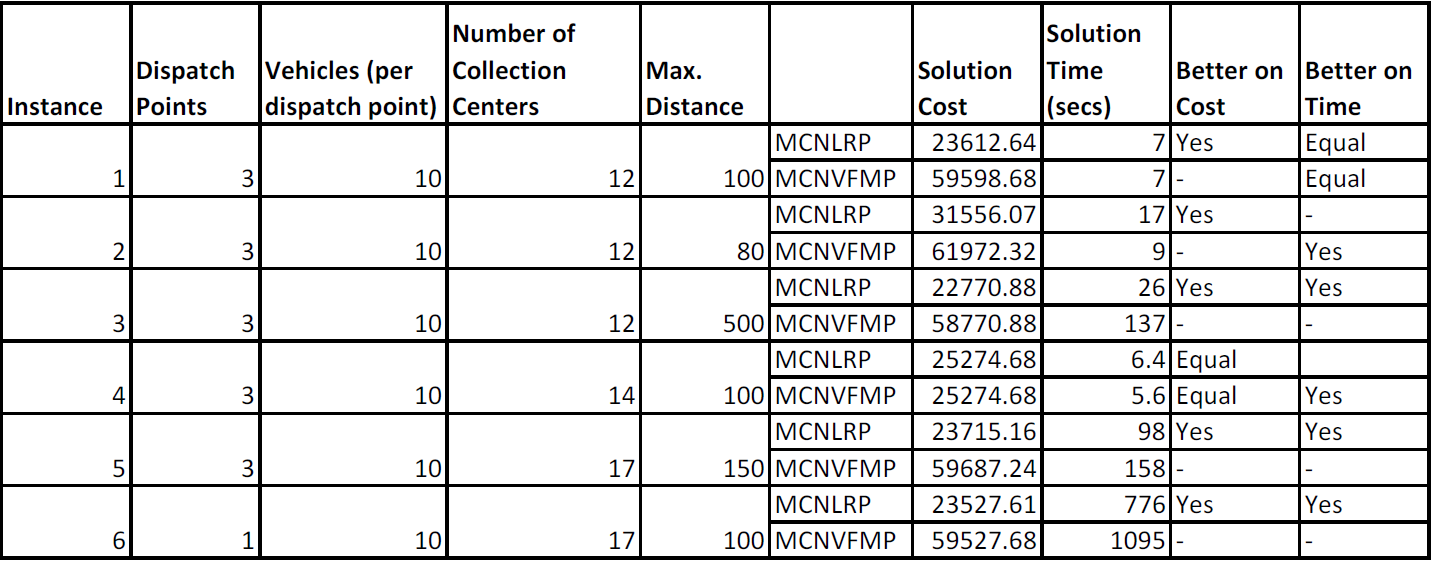
\includegraphics[width=1\textwidth]{mcnlrp.png}
\caption{Resultados del estudio.}
\label{tabla1}
\end{figure} \\

En general lograron mostrar que MCNLRP funciona mejor en casi todos los casos comparado a MCNVFMP. \\

En 2016 un grupo de investigadores chilenos, Germ\'an Paredes-Belmar, Vladimir Marianov, Andr\'es Bronfman, Carlos Obreque y Armin L\"uer-Villagra llevaron a cabo la resoluci\'on de un MCPB con restricciones, funci\'on objetivo y variables como las que se abordar\'an en este proyecto\cite{MCPB}. Su manera de resoluci\'on fue la de aplicar un modelo mixto de programaci\'on de enteros (mixed integer-programming model), un algoritmo de corte y un algoritmo de ramificaci\'on y corte para la resoluci\'on de problemas de tama\~{n}o mediano, mientras que para problemas de mayores proporciones presentan una heur\'istica de tres etapas que aplican a casos reales. \\

Antes de seguir vale explicar la heur\'istica que aplicaron en este estudio ya que es m\'as interesante debido a que abarca problemas de mayor envergadura. La heur\'istica utilizada se divide entres pasos:
\begin{enumerate}
    \item Dividir el problema en varios problemas m\'as peque\~{n}os utilizando criterios acorde al problema.
    \item A cada cl\'uster se le asigna una cuota de leche para garantizar que se cumplan las restricciones m\'inimas de cada tipo de leche para el problema. Esto se realiza usando una formulaci\'on de programaci\'on de enteros mixtos.
    \item La tercera etapa utiliza el m\'etodo de ramificaci\'on y corte que utilizan para resolver problemas de menor tama\~{n}o.
\end{enumerate} \\

Lo m\'as interesante de este estudio es su aplicaci\'on a un caso real: en la zona sur de Chile. En general los problemas te\'oricos consideran las distancias euclidianas entre los nodos para llevar a cabo la resoluci\'on, pero rara vez estas distancias son representativas del mundo real: existen muchas barreras f\'isicas como colinas, monta\~{n}as, r\'ios, lagos, entre otros, que obligan a realizar otros trayectos m\'as costosos que la l\'inea recta que une los nodos. De esta manera la divisi\'on de la zona se llevo alrededor de estas barreras f\'isicas y resultaron finalmente en 25 zonas diferentes. Luego se realizan los pasos 2 y 3, llegando a los resultados mostrados en el Cuadro \ref{chile}.


\begin{table}[H]
\centering
\caption{Resultados para el caso real de Chile.}
\label{chile}
\resizebox{\textwidth}{!}{%
\begin{tabular}{|l|l|l|l|}
\hline
                              & MB            & VRP         & Current Procedure \\ \hline
Trucks                        & 81            & 99          & 100               \\ \hline
Revenue{[}MU{]}               & 23,266        & 24,273      & 22,804            \\ \hline
Costs{[}MU{]}                 & 10,093        & 12,319      & 18,659            \\ \hline
Profit{[}MU{]}                & 13,173        & 11,954      & 4145              \\ \hline
Milk A{[}l{]}                 & 1,278,815     & 1,435,168   & 1,051,791         \\ \hline
Milk B{[}l{]}                 & 306,060       & 268,564     & 627,043           \\ \hline
Milk B{[}l{]}                 & 193,332       & 74,475      & 99,373            \\ \hline
A -\textgreater B {[}l{]}     & 0             & 31,436      & -                 \\ \hline
A -\textgreater C {[}l{]}     & 0             & 25,525      & -                 \\ \hline
B -\textgreater C {[}l{]}     & 0             & -           & 627               \\ \hline
CPU time (clock time) {[}s{]} & 23,836 (5959) & 6241 (1560) & -                 \\ \hline
\end{tabular}%
}
\end{table}

A partir de esta tabla se puede ver una disminuci\'on en la cantidad de camiones requeridos (y, por ende, cantidad de rutas) para la recolecci\'on, como tambi\'en un aumento de la ganancia al final del d\'ia. No obstante, todo esto es a expensas de un mayor tiempo para encontrar esta soluci\'on \'optima. \\

Avanzando con el paper ya mencionado de Sethanan y Pitakaso donde resuelven el problema para camiones que cuentan con varios compartimientos para no mezclar la leche y con puntos de recolecci\'on (o puntos de acercamiento de las granjas)\cite{Compartimientos}. Restricciones nuevas aparecen, como tambi\'en nuevos par\'ametros, siendo los m\'as interesantes la limpieza de los camiones y capacidades para cada uno de los compartimientos. En lugar de maximizar alg\'un tipo de beneficio su objetivo es minimizar los costos asociados a todo el proceso. La t\'ecnica de resoluci\'on que utilizan para resolver el problema es el de evoluci\'on diferencial (Diffential evolution, DE). Esta t\'ecnica optimiza el problema de manera iterativa, ofreciendo un candidato para la soluci\'on y luego mejorando este candidato hasta que no exista ninguno mejor. De manera general, este algoritmo funciona de la siguiente manera:
\begin{enumerate}
    \item Generar soluci\'on inicial.
    \item Realizar el proceso de mutaci\'on.
    \item Realizar el proceso de recombinaci\'on.
    \item Realizar el proceso de selecci\'on.
\end{enumerate}

Para mejorar a\'un m\'as el algoritmo, Sethanan y Pitakaso propusieron a\~{n}adir dos pasos m\'as:
\begin{enumerate}
    \item Proceso de reencarnaci\'on.
    \item Proceso de supervivencia.
\end{enumerate}

En la Figura \ref{process} se puede ver como queda este algoritmo.

\begin{figure}[H]
\centering
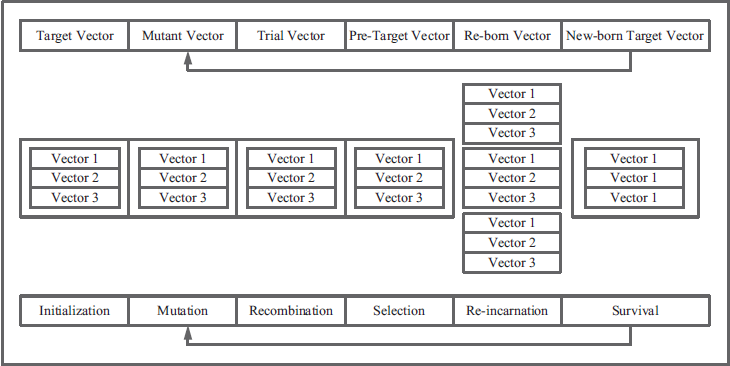
\includegraphics[width=1\textwidth]{Screenshot_1.png}
\caption{Algoritmo modificado.}
\label{process}
\end{figure} \\

Existe una gran complejidad en la descripci\'on del paso a paso de este problema, pero finalmente se desmuestra que el DE modificado da mejores resultados que el DE tradicional no solamente reduciendo los costos del problema, sino tambi\'en en la administraci\'on eficiente del n\'umero de camiones usados. \\

M\'as adelante, en 2017, algunos de los investigadores mencionados en el estudio anterior participaron de otro trabajo en el cual resuelven el problema MCPB con puntos de recolecci\'on \cite{puntos}. El problema considera camiones sin compartimientos donde puede existir mezcla de leche degradando la de m\'as alto grado. En esta cuesti\'on tambi\'en se busca determinar en d\'onde deber\'ian estar ubicados los puntos de recolecci\'on y qu\'e granjas deber\'ian participar en estos. El acercamiento que tuvieron a este desafi\'io fue en torno a un modelo de programaci\'on de enteros y dos estrategias de implementaci\'on: un algoritmo de ramificaci\'on y corte para instancias peque\~{n}as y para casos mayores una heur\'istica que combina m\'etodos exactos y aproximados. Adem\'as, realizan la aplicaci\'on para un caso real utilizando 500 granjas y 112 posibles puntos de recolecci\'on. \\

Como se menciona anteriormente, el problema m\'as interesante es para casos de gran escala donde existen muchas granjas que entregan leche. Para estos problemas ofrecen una heur\'istica que consiste en tres etapas mostradas en la Figura \ref{process2}.

\begin{figure}[H]
\centering
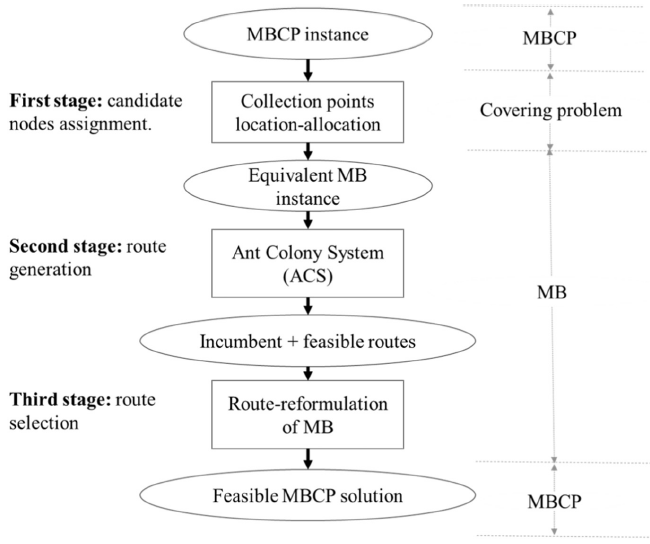
\includegraphics[width=1\textwidth]{Screenshot_2.png}
\caption{Heur\'istica de 3 etapas propuesta.}
\label{process2}
\end{figure} \\

Esta t\'ecnica de resoluci\'on se entrega para resolver la recolecci\'on en zonas rurales donde existen muchas granjas peque\~{n}as a lo largo de toda la regi\'on. Los m\'etodos propuestos mostraron una disminuci\'on del costo total colocando puntos de recolecci\'on donde los productores de leche pueden llevar su leche si es que el costo de ese transporte es menor al de ir a recolectar la leche directamente a la granja. No obstante, al aplicar sus m\'etodos a un caso real, si bien se ve que disminuyen costos y aumentan las ganancias, el tiempo que demora en poder encontrar la soluci\'on \'optima es considerablemente mayor que otros m\'etodos, aunque cabe destacar que cuando existe mezcla y puntos de recolecci\'on en el problema aumentan considerablemente las ganancias y disminuyen bastante los costos, por lo que se debe analizar en mayor profundidad la aplicabilidad de estos m\'etodos. \\

En su tesis de pregrado, Diego Escobar Boehmwald utiliza un algoritmo gen\'etico para resolver el problema de recolecci\'on de leche \cite{genetico}. Este algoritmo cuenta con 4 etapas:
\begin{enumerate}
    \item Fase de construcci\'on, donde a trav\'es de alguna t\'ecnica se genera la primera generaci\'on de soluci\'on.
    \item Etapa de transformaci\'on (cruzamiento y mutaci\'on).
    \item Elitismo, donde se eval\'ua la calidad de las soluciones obtenidas y se identifican y almacenan las mejores soluciones para la siguiente generaci\'on.
    \item Selecci\'on.
\end{enumerate}

Estas etapas se repiten, mejorando la poblaci\'on de soluciones en cada generaci\'on hasta alcanzar la soluci\'on \'optima. Esta soluci\'on se va alcanzando en base a las generaciones pasadas. En su tesis el objetivo principal es el disminuir los costos de la recolecci\'on que incluyen el costo de la recolecci\'on de la leche en si y el costo de combustible. Adem\'as, especifica las siguientes finalidades:
\begin{enumerate}
    \item Comprobar la efectividad en el desempe\~{n}o del algoritmo.
    \item Comparar las heur\'isticas de selecci\'on de componentes en el algoritmo de generaci\'on de soluciones iniciales.
    \item Comparaci\'on con el estado del arte.
\end{enumerate}

Los resultados obtenidos fueron satisfactorios, pero se aprecia que existen (seg\'un el autor) varias maneras de mejorar el algoritmo y las t\'ecnicas para obtener mejores resultados.

\section{Modelo Matem\'atico}

Como se mencion\'o en secciones anteriores, el problema a resolver aqu\'i quiz\'a sea un poco m\'as simplificado comparado con los vistos en el Estado del Arte. Ahora se llevar\'a a cabo la traducci\'on de los par\'ametros, variables, restricciones y objetivos del problema a un modelo matem\'atico.

\subsection{Par\'ametros}

\begin{itemize}
    \item $A$: es el conjunto de arcos (caminos) que unen las granjas de leche.
    \item $A^0$: es el conjunto de arcos (caminos) que unen las granjas con la planta.
    \item $N = $ $\{0,1,...,n\}$ granjas de leche
    \item $N_0$: conjunto de granjas y la planta.
    \item $K$: conjunto de camiones.
    \item $T$: conjunto de calidades de leche.
    \item $N^t$: conjunto de granjas de leche de calidad $t \: \in \: T$.
    \item $D^t$: resultado de la mezcla de leche de calidad $r$ con leche de calidad $t$.
    \item $IT$: conjunto de pares ordenados $(i,t)$ de granjas $i$ y leche de calidad $t$, donde cada granja solo produce una calidad de leche.
    \item $Q^k$: capacidad de cada cami\'on $k$.
    \item $q^t_i$: cantidad de leche $t$ producida por la granja $i$.
    \item $c^k_{ij}$: costo de viaje de cada cami\'on $k$ sobre el arco $(i,j) \: \in \: A \cup A^0$.
    \item $\alpha^t$: ingreso por unidad de leche de calidad $t$.
    \item $P^t$: requerimientos de leche de calidad $t$ de la planta.
    \item $K_i = $ $\{k \: \in \: K \:: \: t \: \in \: T,q^t_i \leq Q^k \: \forall t\}$ Conjunto de camiones que pueden visitar la granja $i$.
    \item $K_{ij} = $ $\{k \: \in \: K \:: \: q^t_i + q^t_j \leq Q^k \: \forall t\}$ Conjunto de camiones que pueden viajar de la granja $i$ a la granja $j$ recolectando la leche que ambas granjas producen sin exceder la capacidad del cami\'on, para cada arco $(i,j) \: \in \: A \cup A^0$.
    \item $0_k$: nodo en el que el cami\'on $k$ inicia la ruta.
    \item $AK =$ $\{(i,j,k) \:: \: (i,j) \: \in \: A \cup A^0,k \: \in \: K_{ij}\}$ Conjunto de elementos que contiene un arco que va de la granja $i$ a la granja $j$ y un cami\'on $k$ que pertenece a $K_{ij}$.
\end{itemize}

\subsection{Variables de decisi\'on}

\subsubsection{Variables de tipo binaria}

\begin{equation*}
    x^k_{ij} = \left\{\begin{array}{lr}
        1, \text{Si el cami\'on k viaja directamente del nodo i al nodo j }\\
        0, \text{en caso contrario}
        \end{array}
        \right
\end{equation*}

\begin{equation*}
    y^{kt}_i = \left\{\begin{array}{lr}
        1, \text{Si el cami\'on k recoge leche de calidad t de la granja i }\\
        0, \text{en caso contrario}
        \end{array}\right 
\end{equation*}

\begin{equation*}
    z^{kt} = \left\{\begin{array}{lr}
        1, \text{Si el cami\'on k entrega leche de calidad t a la planta }\\
        0, \text{en caso contrario}
        \end{array}\right 
\end{equation*}

\subsubsection{Variables de control de cantidad de leche entregada}
\begin{align*} 
w^{kt} &= \text{Volumen de leche de calidad t que el cami\'on k entrega a la planta.} \\
v^{tr} &= \text{Volumen de leche de calidad t entregada a la planta, mezclada para su uso como leche de calidad r.}
\end{align*}

\subsection{Restricciones}

\begin{itemize}
    \item Los camiones no pueden llevar m\'as leche que su capacidad m\'axima.
    
    \begin{equation}
        \sum_{t \in T} \sum_{i \in N : (i,j) \in IT} q_i^t y^{kt}_i \leq Q^k, \: \forall k \in K
    \end{equation}
    
     \item La leche de cada granja debe ser recolectada exactamente por solo 1 cami\'on.
     
     \begin{equation}
         \sum_{k \in K_i} y_i^{kt} = 1, \: \forall i \in N, t \in T \:: (i,j) \in IT
     \end{equation}
     
     \item Cada cami\'on solo debe realizar una ruta que comienza en alg\'un nodo $0_k$ para cada cami\'on $k$.
     
     \begin{equation}
         \sum_{j:(0_k,j,k) \in AK} x^k_{0kj} \leq 1, \: \forall k \in K 
     \end{equation}
     
     \item Orden en el flujo de cada cami\'on y cada nodo.
     
     \begin{equation}
         \sum_{i:(i,j,k)\in AK} x^k_{ij} = \sum_{h:(j,h,k)\in AK} x^k_{jh}, \: \forall k \in K_j,\: j \in N_0
     \end{equation}
     
     \item Si un cami\'on $k$ en su ruta debe detenerse en el nodo $i$ a recolectar la leche.
     
     \begin{equation}
         \sum_{p:(p,i,k)\in AK} x^k_{pi} = y^{kt}_i, \: \forall k \in K_i, i \in N, t \in T : (i,t) \in IT
     \end{equation}
     
     \item Si el cami\'on $k$ debe llevar leche de calidad $t$ a la planta, entonces no puede recolectar leche de menor calidad a $t$.
     
     \begin{equation}
         z^{kt} \leq 1 - \sum_{\substack{r \in D^t : r \neq t \\ (i,r) \in IT}} y^{kr}_i, \: \forall k \in K_i, i \in N, t \in T
     \end{equation}
     
     \item Cada cami\'on $k$ solo debe entregar un tipo de leche a la granja (puede ser mezclada).
     
     \begin{equation}
         \sum_{t \in T} z^{kt} \leq 1, \: \forall k \in K
     \end{equation}
     
     \item La cantidad de leche entregada de cada tipo por cada cami\'on a la planta no supera su capacidad.
     
     \begin{equation}
         w^{kt} \leq z^{kt}Q^k, \: \forall k \in K, t \in T
     \end{equation}
     
     \item La cantidad recolectada de cada tipo de leche por cada cami\'on no supera su capacidad.
     
     \begin{equation}
         w^{kt} \leq \sum_{r:i \in D^r} \sum_{h \in N^r} q^r_h y^{kr}_h, \: \forall k \in K, t \in T
     \end{equation}
     
     \item Toda la leche recolectada debe ser llevada a la planta.
     
     \begin{equation}
         \sum_{k \in K} \sum_{t \in T} w^{kt} = \sum_{(i,t) \in IT} q^t_i
     \end{equation}
     
     \item Se debe equilibrar la cantidad de leche de cada calidad que llega a la planta y la cantidad de leche de cada calidad restante despu\'es de la mezcla en la planta.
     
     \begin{equation}
         \sum_{r \in D^t} v^{tr} = \sum_{k \in K} w^{kt}, \: \forall t \in T
     \end{equation}
     
     \item Se deben satisfacer las cuotas de cada tipo de leche.
     
     \begin{equation}
         \sum_{t \in T} v^{tr} \geq P^r, \: \forall r \in D^t
     \end{equation}
     
     \item No se pueden mezclar ciertas leches.
     
     \begin{equation}
         y^{kt}_i + y^{kr}_i \leq 1, \: \forall (t,r) \in PM; (i,t),(j,t) \in IT
     \end{equation}
     
     \item No pueden existir sub-ciclos en las rutas de los camiones.
     
     \begin{equation}
         \sum_{i \in S} \sum_{j \in S} x^k_{ij} \leq |S| - 1, \: \forall S \subseteq N, k \in K
     \end{equation}
     
     \item Naturaleza de las variables.
     
     \begin{equation}
         y^{kt}_i, z^{kt} \in \{0,1\} \: \forall i \in N, k \in K_i, t \in T : (i,t) \in IT
     \end{equation}
     
     \begin{equation}
         x^k_{ij} \in \{0,1\} \: \forall (i,j,k) \in AK
     \end{equation}
     
     \begin{equation}
         w^{kt}, v^{tr} \geq 0, \: \forall k \in K; t, r \in T, r \in D^t
     \end{equation}
\end{itemize}

\subsection{Funci\'on objetivo}

Para el problema del proyecto se busca maximizar la utilidad final obtenida de la recolecci\'on de leche, por lo que en la funci\'on objetivo intervienen las ganancias generadas por la leche recolectada y el gasto asociado al transporte de esta.

\begin{equation*}
    \text{Max} \sum_{t \in T} \sum_{r \in T} \alpha^r v^{tr} - \sum_{(i,j,k) \in AK} c^k_{ij} x^k_{ij}
\end{equation*}

Entre la documentaci\'on encontrada, este problema corresponde al mismo analizado por el grupo de estudiantes chilenos mencionado en el Estado del Arte \cite{MCPB}.


\section{Representaci\'on}

En primer lugar, como se trabajó en lenguaje de programación C++, se aprovechó de su orientación a objetos y se creó la clase \textit{camión} que representa a los distintos camiones que van a recolectar leche. De esta manera es más simple contener la información de los camiones, tales como nodos visitados, distancia recorrida, utilidad generada, capacidad utilizada, entre otros, que tenerlas en arreglos o vectores separados de los objetos. Por otra parte, se utiliza una gran cantidad de vectores para contener datos interesantes, tales como:

\begin{itemize}
    \item Capacidad de los camiones.
    \item Ganancia generada por cada tipo de leche.
    \item Nodos.
    \item Posiciones de los nodos.
    \item Tipo de leche generada por cada nodo (es una matriz).
    \item Cantidad de leche generada por cada nodo.
    \item Distancias entre los nodos (es una matriz)
    \item Camiones.
\end{itemize}

La razón del gran uso de vectores es porque no se conoce a priori la cantidad de los elementos antes mencionados, por lo cual definir arreglos se vuelve más complejo y es mejor utilizar vectores. Además, es más fácil manejar las restricciones con respecto a las calidades de las leches. \\

La solución final del problema se entrega como un vector de camiones. Cada camión posee un vector con los nodos que visitó, excluyendo al nodo 1 (el nodo de la planta) ya que todos deben ir y llegar a este, por lo cual no tiene sentido colocarlo en sus nodos visitados. Además, tienen la información de la distancia recorrida y de la utilidad generada. \\

\section{Descripci\'on del algoritmo}

El algoritmo evolutivo implementado sigue el típico esquema que se ha visto en clases:

\begin{lstlisting}
    t = 0;
    inicializar(P(t=0));
    evaluar(P(t=0));
    solución(mejor(P))
    while(t<t_final):
        Cruzamiento(con probabilidad Pc);
        Mutacion(con probabilidad Pm);
        evaluar(P(t=t'));
        solucion(mejor(actual,P'));
        t++;
    end
\end{lstlisting}

A continuación, se explicarán la implementación de las distintas partes de este algoritmo.

\subsection{Generación de solución inicial}

Para generar la población inicial se utilizaron las siguientes heurísticas:
\begin{itemize}
    \item Completamente aleatoria.
    \item Se le asigna el camión más grande al requerimiento de leche más grande.
    \item La población será de 50 posibles soluciones (recordad que cada solución tiene 3 camiones en este caso).
\end{itemize}

De esta población inicial se obtiene la mejor solución actual y se guarda en una variable dentro del programa. A partir de esta población inicial se generarán las siguientes generaciones en el algoritmo evolutivo.

\subsection{Etapa de cruzamiento}

La técnica utilizada en el cruzamiento fue la de cruzamiento en un punto, vale decir, se hace un corte en ambos individuos y se intercambian su código genético, generando así dos hijos a partir de dos padres. Cosas a tener en consideración:

\begin{itemize}
    \item La probabilidad de cruzamiento es, arbitrariamente, de 80\%.
    \item Como cada individuo consta de 3 camiones, el cruzamiento se hace con los camiones que portan la misma leche, vale decir, no se puede hacer cruzamiento entre un camion que lleve leche final tipo B y otro que lleve leche final tipo C, por ejemplo.
    \item Si los individuos tienen largo diferentes (los largos vienen dados por los nodos visitados), entonces se utiliza al más pequeño como base para hacer el corte.
    \item Como existe la posibilidad de que algún individuo, tras el cruzamiento, visite un nodo más de una vez, fue necesario implementar una función que detectara estos nodos repetidos, revisara los nodos disponibles para visitar y los reemplazara.
\end{itemize}

\subsection{Etapa de mutación}

Para la etapa de mutación también se mantuvo la simplicidad y lo que se hizo fue el intercambio de dos nodos en el orden de visita del camión. En otras palabras, se quitan 4 arcos y se reemplazan con 4 arcos diferentes. Cosas a tener en consideración:

\begin{itemize}
    \item La probabilidad de mutación es, arbitrariamente, de 5\%.
    \item Si existe mutación, TODOS los camiones del individuo mutan.
\end{itemize}

\subsection{Etapa de evaluación}

Tras haber hecho todos los cruzamientos y mutaciones correspondientes, a estos nuevos inidividuos se le deben calcular varios elementos:

\begin{itemize}
    \item Distancia recorrida.
    \item Cantidad de leche recolectada.
    \item Utilidad generada.
\end{itemize}

La mejor solución siempre se mantiene guardada en un vector que solo es modificado si aparece una solución igual o mejor, por lo que una solución podría perdurar por varias generaciones. De esta forma, tras realizar los cálculos descritos anteriormente, se verifica cual es la mejor solución del conjunto y se compara con la mejor solución actualmente guardada, reemplazándola en el caso de que la mejor solución de la población actual se igual o mejor a ella.

\section{Experimentos}

Debido a que es una técnica incompleta, no existe algún criterio general para poder definir el tamaño de la población, el cual es un factor muy relevante al momento de plantear un algoritmo evolutivo. Por lo tanto, los experimentos fueron realizados variando la cantidad de iteraciones y el tamaño de la población. \\

A pesar de los esfuerzos por poder solucionar todas las instancias entregadas para este proyecto, no se lograron realizar en su completitud. La razón de esto recae en aquellas instancias donde la cantidad de nodos no es múltiplo del número de camiones (sin contar a la planta) ya que quedan soluciones con largos diferentes y al hacer el cruzamiento se generan problemas ya que uno de los individuos puede quedar con muchas copias mientras que el otro tiene pocas o nulas copias (con copias me refiero a nodos repetidos). Una forma teórica de solucionar esto es con un vector global entre los 6 camiones (es decir, ambos individuos) que permita discernir qué nodos están disponibles para visitar, pero como se está contra el tiempo no se alcanzó a realizar. Es así como las instancias que se utilizaron para probar la aplicación son aquellos que poseen una cantidad de nodos múltiplo de 3 + 1. \\

Los parámetros que se variaron fueron:

\begin{itemize}
    \item Tamaño de la población (50 y 100).
    \item Número de iteraciones (100, 1000 y 10000).
\end{itemize}

Aunque todos estos parámetros se podrían pedir al momento de ejecutar el programa, se decidió dejar las especificaciones iniciales de que solo el número de iteraciones (junto al archivo .txt) es ingresado por el usuario, ya que el ingresar muchos parámetros puede ser tedioso, además de llevar a un error de ingresar en orden incorrecto los valores. \\

Los bugs y el seguimiento de los valores de las variables fueron llevados a cabo a través del depurador GDB y con la (mala) práctica de los \textit{prints}.\\

De esta manera, las configuraciones utilizadas para probrar el programa fueron:

\begin{itemize}
    \item Configuración 1
    
    \begin{itemize}
        \item Tamaño de la población: 50.
        \item Número de iteraciones: 100.
    \end{itemize}
    
    \item Configuración 2
    
    \begin{itemize}
        \item Tamaño de la población: 50.
        \item Número de iteraciones: 1000.
    \end{itemize}
    
    \item Configuración 3
    
    \begin{itemize}
        \item Tamaño de la población: 50.
        \item Número de iteraciones: 10000.
    \end{itemize}
    
    \item Configuración 4
    
    \begin{itemize}
        \item Tamaño de la población: 100.
        \item Número de iteraciones: 100.
    \end{itemize}
    
    \item Configuración 5
    
    \begin{itemize}
        \item Tamaño de la población: 100.
        \item Número de iteraciones: 1000.
    \end{itemize}
    
    \item Configuración 6
    
    \begin{itemize}
        \item Tamaño de la población: 100.
        \item Número de iteraciones: 10000.
    \end{itemize}
\end{itemize}

\section{Resultados}

% Please add the following required packages to your document preamble:
% \usepackage{multirow}
% \usepackage{longtable}
% Note: It may be necessary to compile the document several times to get a multi-page table to line up properly
\begin{longtable}[c]{|c|c|l|l|l|l|l|l|l|}
\hline
\multicolumn{1}{|l|}{\begin{tabular}[c]{@{}l@{}}Tamaño \\ Población\end{tabular}} & \multicolumn{1}{l|}{Iteraciones} & Pc {[}\%{]} & Instancia & \begin{tabular}[c]{@{}l@{}}Tipo de \\ leche\end{tabular} & \begin{tabular}[c]{@{}l@{}}Distancia \\ recorrida\end{tabular} & \begin{tabular}[c]{@{}l@{}}Leche \\ recolectada\end{tabular} & Utilidad & Tiempo{[}s{]} \\ \hline
\endfirsthead
%
\endhead
%
\multirow{24}{*}{50} & \multirow{8}{*}{100} & 70 & a55.txt & \begin{tabular}[c]{@{}l@{}}A\\ B\\ C\end{tabular} & \begin{tabular}[c]{@{}l@{}}924.057\\ 611.231\\ 889.378\end{tabular} & \begin{tabular}[c]{@{}l@{}}11900\\ 12250\\ 17800\end{tabular} & 23390.3 & 1.6 \\ \cline{3-9} 
 &  & 70 & a64.txt & \begin{tabular}[c]{@{}l@{}}A\\ B\\ C\end{tabular} & \begin{tabular}[c]{@{}l@{}}1072.88\\ 875.295\\ 771.332\end{tabular} & \begin{tabular}[c]{@{}l@{}}11750\\ 16000\\ 14650\end{tabular} & 24625.5 & 2.0 \\ \cline{3-9} 
 &  & 70 & eil22.txt & \begin{tabular}[c]{@{}l@{}}A\\ B\\ C\end{tabular} & \begin{tabular}[c]{@{}l@{}}217.466\\ 199.5\\ 250.999\end{tabular} & \begin{tabular}[c]{@{}l@{}}9800\\ 7200\\ 5500\end{tabular} & 15822 & 1.6 \\ \cline{3-9} 
 &  & 70 & eil76.txt & \begin{tabular}[c]{@{}l@{}}A\\ B\\ C\end{tabular} & \begin{tabular}[c]{@{}l@{}}668.895\\ 750.015\\ 746.868\end{tabular} & \begin{tabular}[c]{@{}l@{}}46800\\ 46700\\ 42900\end{tabular} & 90194.2 & 1.44 \\ \cline{3-9} 
 &  & 80 & a55.txt & \begin{tabular}[c]{@{}l@{}}A\\ B\\ C\end{tabular} & \begin{tabular}[c]{@{}l@{}}750.32\\ 689.309\\ 973.071\end{tabular} & \begin{tabular}[c]{@{}l@{}}11900\\ 12250\\ 17800\end{tabular} & 23402.3 & 2.4 \\ \cline{3-9} 
 &  & 80 & a64.txt & \begin{tabular}[c]{@{}l@{}}A\\ B\\ C\end{tabular} & \begin{tabular}[c]{@{}l@{}}817.382\\ 922.875\\ 934.669\end{tabular} & \begin{tabular}[c]{@{}l@{}}11750\\ 16000\\ 14650\end{tabular} & 24670.1 & 0.7 \\ \cline{3-9} 
 &  & 80 & eil22.txt & \begin{tabular}[c]{@{}l@{}}A\\ B\\ C\end{tabular} & \begin{tabular}[c]{@{}l@{}}196.826\\ 242.745\\ 215.672\end{tabular} & \begin{tabular}[c]{@{}l@{}}9800\\ 7200\\ 5500\end{tabular} & 15834.8 & 0.6 \\ \cline{3-9} 
 &  & 80 & eil76.txt & \begin{tabular}[c]{@{}l@{}}A\\ B\\ C\end{tabular} & \begin{tabular}[c]{@{}l@{}}736.033\\ 641.948\\ 828.424\end{tabular} & \begin{tabular}[c]{@{}l@{}}46800\\ 46700\\ 42900\end{tabular} & 90153.6 & 1.5 \\ \cline{2-9} 
 & \multirow{8}{*}{1000} & 70 & a55.txt & \begin{tabular}[c]{@{}l@{}}A\\ B\\ C\end{tabular} & \begin{tabular}[c]{@{}l@{}}828.137\\ 719.238\\ 776.151\end{tabular} & \begin{tabular}[c]{@{}l@{}}11900\\ 12250\\ 17800\end{tabular} & 23491.5 & 8.1 \\ \cline{3-9} 
 &  & 70 & a64.txt & \begin{tabular}[c]{@{}l@{}}A\\ B\\ C\end{tabular} & \begin{tabular}[c]{@{}l@{}}871.064\\ 959.95\\ 849.545\end{tabular} & \begin{tabular}[c]{@{}l@{}}11750\\ 16000\\ 14650\end{tabular} & 24664.4 & 4.3 \\ \cline{3-9} 
 &  & 70 & eil22.txt & \begin{tabular}[c]{@{}l@{}}A\\ B\\ C\end{tabular} & \begin{tabular}[c]{@{}l@{}}187.545\\ 182.379\\ 233.117\end{tabular} & \begin{tabular}[c]{@{}l@{}}9800\\ 7200\\ 5500\end{tabular} & 15887 & 4.8 \\ \cline{3-9} 
 &  & 70 & eil76.txt & \begin{tabular}[c]{@{}l@{}}A\\ B\\ C\end{tabular} & \begin{tabular}[c]{@{}l@{}}718.363\\ 694.864\\ 700.674\end{tabular} & \begin{tabular}[c]{@{}l@{}}46800\\ 46700\\ 42900\end{tabular} & 90246.1 & 5.2 \\ \cline{3-9} 
 &  & 80 & a55.txt & \begin{tabular}[c]{@{}l@{}}A\\ B\\ C\end{tabular} & \begin{tabular}[c]{@{}l@{}}740.249\\ 822.094\\ 700.315\end{tabular} & \begin{tabular}[c]{@{}l@{}}11900\\ 12250\\ 17800\end{tabular} & 23552.3 & 4.4 \\ \cline{3-9} 
 &  & 80 & a64.txt & \begin{tabular}[c]{@{}l@{}}A\\ B\\ C\end{tabular} & \begin{tabular}[c]{@{}l@{}}914.949\\ 761.821\\ 949.98\end{tabular} & \begin{tabular}[c]{@{}l@{}}11750\\ 16000\\ 14650\end{tabular} & 24718.2 & 5.9 \\ \cline{3-9} 
 &  & 80 & eil22.txt & \begin{tabular}[c]{@{}l@{}}A\\ B\\ C\end{tabular} & \begin{tabular}[c]{@{}l@{}}199.539\\ 204.597\\ 227.491\end{tabular} & \begin{tabular}[c]{@{}l@{}}9800\\ 7200\\ 5500\end{tabular} & 15858.4 & 3 \\ \cline{3-9} 
 &  & 80 & eil76.txt & \begin{tabular}[c]{@{}l@{}}A\\ B\\ C\end{tabular} & \begin{tabular}[c]{@{}l@{}}711.287\\ 762.722\\ 601.031\end{tabular} & \begin{tabular}[c]{@{}l@{}}46800\\ 46700\\ 42900\end{tabular} & 90285 & 10.0 \\ \cline{2-9} 
 & \multirow{8}{*}{10000} & 70 & a55.txt & \begin{tabular}[c]{@{}l@{}}A\\ B\\ C\end{tabular} & \begin{tabular}[c]{@{}l@{}}732.472\\ 653.479\\ 818.072\end{tabular} & \begin{tabular}[c]{@{}l@{}}11900\\ 12250\\ 17800\end{tabular} & 23611 & 46.8 \\ \cline{3-9} 
 &  & 70 & a64.txt & \begin{tabular}[c]{@{}l@{}}A\\ B\\ C\end{tabular} & \begin{tabular}[c]{@{}l@{}}896.179\\ 802.641\\ 883.368\end{tabular} & \begin{tabular}[c]{@{}l@{}}11750\\ 16000\\ 14650\end{tabular} & 24762.8 & 39.3 \\ \cline{3-9} 
 &  & 70 & eil22.txt & \begin{tabular}[c]{@{}l@{}}A\\ B\\ C\end{tabular} & \begin{tabular}[c]{@{}l@{}}187.545\\ 198.658\\ 204.138\end{tabular} & \begin{tabular}[c]{@{}l@{}}9800\\ 7200\\ 5500\end{tabular} & 15899.7 & 32.3 \\ \cline{3-9} 
 &  & 70 & eil76.txt & \begin{tabular}[c]{@{}l@{}}A\\ B\\ C\end{tabular} & \begin{tabular}[c]{@{}l@{}}709.002\\ 660.407\\ 687.278\end{tabular} & \begin{tabular}[c]{@{}l@{}}46800\\ 46700\\ 42900\end{tabular} & 90303.3 & 50.0 \\ \cline{3-9} 
 &  & 80 & a55.txt & \begin{tabular}[c]{@{}l@{}}A\\ B\\ C\end{tabular} & \begin{tabular}[c]{@{}l@{}}919.041\\ 659.376\\ 682.163\end{tabular} & \begin{tabular}[c]{@{}l@{}}11900\\ 12250\\ 17800\end{tabular} & 23554.4 & 39.01 \\ \cline{3-9} 
 &  & 80 & a64.txt & \begin{tabular}[c]{@{}l@{}}A\\ B\\ C\end{tabular} & \begin{tabular}[c]{@{}l@{}}786.888\\ 917.545\\ 856.971\end{tabular} & \begin{tabular}[c]{@{}l@{}}11750\\ 16000\\ 14650\end{tabular} & 24783.6 & 43.1 \\ \cline{3-9} 
 &  & 80 & eil22.txt & \begin{tabular}[c]{@{}l@{}}A\\ B\\ C\end{tabular} & \begin{tabular}[c]{@{}l@{}}205.861\\ 182.512\\ 214.483\end{tabular} & \begin{tabular}[c]{@{}l@{}}9800\\ 7200\\ 5500\end{tabular} & 15887.1 & 30.5 \\ \cline{3-9} 
 &  & 80 & eil76.txt & \begin{tabular}[c]{@{}l@{}}A\\ B\\ C\end{tabular} & \begin{tabular}[c]{@{}l@{}}631.686\\ 729.463\\ 700.153\end{tabular} & \begin{tabular}[c]{@{}l@{}}46800\\ 46700\\ 42900\end{tabular} & 90298.7 & 54.3 \\ \hline
\multirow{24}{*}{100} & \multirow{8}{*}{100} & 70 & a55.txt & \begin{tabular}[c]{@{}l@{}}A\\ B\\ C\end{tabular} & \begin{tabular}[c]{@{}l@{}}794.694\\ 653.835\\ 1012.22\end{tabular} & \begin{tabular}[c]{@{}l@{}}11900\\ 12250\\ 17800\end{tabular} & 23354.2 & 1.8 \\ \cline{3-9} 
 &  & 70 & a64.txt & \begin{tabular}[c]{@{}l@{}}A\\ B\\ C\end{tabular} & \begin{tabular}[c]{@{}l@{}}920.062\\ 951.601\\ 878.007\end{tabular} & \begin{tabular}[c]{@{}l@{}}11750\\ 16000\\ 14650\end{tabular} & 24595.3 & 2.8 \\ \cline{3-9} 
 &  & 70 & eil22.txt & \begin{tabular}[c]{@{}l@{}}A\\ B\\ C\end{tabular} & \begin{tabular}[c]{@{}l@{}}213.38\\ 205.918\\ 209.554\end{tabular} & \begin{tabular}[c]{@{}l@{}}9800\\ 7200\\ 5500\end{tabular} & 15861.1 & 0.8 \\ \cline{3-9} 
 &  & 70 & eil76.txt & \begin{tabular}[c]{@{}l@{}}A\\ B\\ C\end{tabular} & \begin{tabular}[c]{@{}l@{}}689.908\\ 730.784\\ 715.69\end{tabular} & \begin{tabular}[c]{@{}l@{}}46800\\ 46700\\ 42900\end{tabular} & 90223.6 & 1.3 \\ \cline{3-9} 
 &  & 80 & a55.txt & \begin{tabular}[c]{@{}l@{}}A\\ B\\ C\end{tabular} & \begin{tabular}[c]{@{}l@{}}845.18\\ 691.305\\ 851.037\end{tabular} & \begin{tabular}[c]{@{}l@{}}11900\\ 12250\\ 17800\end{tabular} & 23427.5 & 1.0 \\ \cline{3-9} 
 &  & 80 & a64.txt & \begin{tabular}[c]{@{}l@{}}A\\ B\\ C\end{tabular} & \begin{tabular}[c]{@{}l@{}}964.055\\ 820.748\\ 970.099\end{tabular} & \begin{tabular}[c]{@{}l@{}}11750\\ 16000\\ 14650\end{tabular} & 24590.1 & 6.0 \\ \cline{3-9} 
 &  & 80 & eil22.txt & \begin{tabular}[c]{@{}l@{}}A\\ B\\ C\end{tabular} & \begin{tabular}[c]{@{}l@{}}236.665\\ 203.922\\ 220.84\end{tabular} & \begin{tabular}[c]{@{}l@{}}9800\\ 7200\\ 5500\end{tabular} & 15828.6 & 2.6 \\ \cline{3-9} 
 &  & 80 & eil76.txt & \begin{tabular}[c]{@{}l@{}}A\\ B\\ C\end{tabular} & \begin{tabular}[c]{@{}l@{}}692.863\\ 753.528\\ 710.764\end{tabular} & \begin{tabular}[c]{@{}l@{}}46800\\ 46700\\ 42900\end{tabular} & 90202.8 & 2.4 \\ \cline{2-9} 
 & \multirow{8}{*}{1000} & 70 & a55.txt & \begin{tabular}[c]{@{}l@{}}A\\ B\\ C\end{tabular} & \begin{tabular}[c]{@{}l@{}}790.474\\ 780.844\\ 706.573\end{tabular} & \begin{tabular}[c]{@{}l@{}}11900\\ 12250\\ 17800\end{tabular} & 23537.1 & 9.8 \\ \cline{3-9} 
 &  & 70 & a64.txt & \begin{tabular}[c]{@{}l@{}}A\\ B\\ C\end{tabular} & \begin{tabular}[c]{@{}l@{}}989.738\\ 754.496\\ 864.196\end{tabular} & \begin{tabular}[c]{@{}l@{}}11750\\ 16000\\ 14650\end{tabular} & 24736.6 & 13.0 \\ \cline{3-9} 
 &  & 70 & eil22.txt & \begin{tabular}[c]{@{}l@{}}A\\ B\\ C\end{tabular} & \begin{tabular}[c]{@{}l@{}}196.826\\ 180.771\\ 233.549\end{tabular} & \begin{tabular}[c]{@{}l@{}}9800\\ 7200\\ 5500\end{tabular} & 15878.9 & 8.2 \\ \cline{3-9} 
 &  & 70 & eil76.txt & \begin{tabular}[c]{@{}l@{}}A\\ B\\ C\end{tabular} & \begin{tabular}[c]{@{}l@{}}717.97\\ 695.592\\ 654.251\end{tabular} & \begin{tabular}[c]{@{}l@{}}46800\\ 46700\\ 42900\end{tabular} & 90292.2 & 13.0 \\ \cline{3-9} 
 &  & 80 & a55.txt & \begin{tabular}[c]{@{}l@{}}A\\ B\\ C\end{tabular} & \begin{tabular}[c]{@{}l@{}}770.294\\ 799.624\\ 734.174\end{tabular} & \begin{tabular}[c]{@{}l@{}}11900\\ 12250\\ 17800\end{tabular} & 23510.9 & 8.0 \\ \cline{3-9} 
 &  & 80 & a64.txt & \begin{tabular}[c]{@{}l@{}}A\\ B\\ C\end{tabular} & \begin{tabular}[c]{@{}l@{}}694.624\\ 1046.47\\ 828.235\end{tabular} & \begin{tabular}[c]{@{}l@{}}11750\\ 16000\\ 14650\end{tabular} & 24775.7 & 10.8 \\ \cline{3-9} 
 &  & 80 & eil22.txt & \begin{tabular}[c]{@{}l@{}}A\\ B\\ C\end{tabular} & \begin{tabular}[c]{@{}l@{}}191.607\\ 181.959\\ 235.233\end{tabular} & \begin{tabular}[c]{@{}l@{}}9800\\ 7200\\ 5500\end{tabular} & 15881.2 & 12.3 \\ \cline{3-9} 
 &  & 80 & eil76.txt & \begin{tabular}[c]{@{}l@{}}A\\ B\\ C\end{tabular} & \begin{tabular}[c]{@{}l@{}}598.214\\ 824.311\\ 605.97\end{tabular} & \begin{tabular}[c]{@{}l@{}}46800\\ 46700\\ 42900\end{tabular} & 90331.5 & 16.3 \\ \cline{2-9} 
 & \multirow{8}{*}{10000} & 70 & a55.txt & \begin{tabular}[c]{@{}l@{}}A\\ B\\ C\end{tabular} & \begin{tabular}[c]{@{}l@{}}739.531\\ 608.086\\ 865.564\end{tabular} & \begin{tabular}[c]{@{}l@{}}11900\\ 12250\\ 17800\end{tabular} & 23601.8 & 78.1 \\ \cline{3-9} 
 &  & 70 & a64.txt & \begin{tabular}[c]{@{}l@{}}A\\ B\\ C\end{tabular} & \begin{tabular}[c]{@{}l@{}}796.462\\ 1034.43\\ 742.899\end{tabular} & \begin{tabular}[c]{@{}l@{}}11750\\ 16000\\ 14650\end{tabular} & 24771.2 & 82.0 \\ \cline{3-9} 
 &  & 70 & eil22.txt & \begin{tabular}[c]{@{}l@{}}A\\ B\\ C\end{tabular} & \begin{tabular}[c]{@{}l@{}}189.058\\ 206.606\\ 201.206\end{tabular} & \begin{tabular}[c]{@{}l@{}}9800\\ 7200\\ 5500\end{tabular} & 15893.1 & 64.6 \\ \cline{3-9} 
 &  & 70 & eil76.txt & \begin{tabular}[c]{@{}l@{}}A\\ B\\ C\end{tabular} & \begin{tabular}[c]{@{}l@{}}579.429\\ 726.299\\ 712.351\end{tabular} & \begin{tabular}[c]{@{}l@{}}46800\\ 46700\\ 42900\end{tabular} & 90341.9 & 117.4 \\ \cline{3-9} 
 &  & 80 & a55.txt & \begin{tabular}[c]{@{}l@{}}A\\ B\\ C\end{tabular} & \begin{tabular}[c]{@{}l@{}}736.039\\ 716.394\\ 759.687\end{tabular} & \begin{tabular}[c]{@{}l@{}}11900\\ 12250\\ 17800\end{tabular} & 23602.9 & 77.7 \\ \cline{3-9} 
 &  & 80 & a64.txt & \begin{tabular}[c]{@{}l@{}}A\\ B\\ C\end{tabular} & \begin{tabular}[c]{@{}l@{}}851.648\\ 821.405\\ 890.518\end{tabular} & \begin{tabular}[c]{@{}l@{}}11750\\ 16000\\ 14650\end{tabular} & 24781.4 & 83.4 \\ \cline{3-9} 
 &  & 80 & eil22.txt & \begin{tabular}[c]{@{}l@{}}A\\ B\\ C\end{tabular} & \begin{tabular}[c]{@{}l@{}}205.861\\ 189.176\\ 201.206\end{tabular} & \begin{tabular}[c]{@{}l@{}}9800\\ 7200\\ 5500\end{tabular} & 15893.8 & 55.8 \\ \cline{3-9} 
 &  & 80 & eil76.txt & \begin{tabular}[c]{@{}l@{}}A\\ B\\ C\end{tabular} & \begin{tabular}[c]{@{}l@{}}781.403\\ 591.574\\ 648.975\end{tabular} & \begin{tabular}[c]{@{}l@{}}46800\\ 46700\\ 42900\end{tabular} & 90338 & 117.9 \\ \hline
\end{longtable}

A partir de la tabla anterior se puede ver que un cambio entre entre 70\% y 80\% no tiene una clara incidencia en el resultado final, ya que en algunos casos una probabilidad de cruzamiento de 80\% obtiene mayores utilidades, pero en otros casos el de 70\% obtiene mejores resultados, por lo cual no se puede llegar a una conclusión con respecto a esto. Arbitrariamente se dejará la probabilidad de cruzamiento como 80\%. \\

Analizando las otras variables, a continuación se presenta un gráfico del tiempo que toma al algoritmo en terminar su ejecución vs la cantidad de nodos para el caso de una población de 50 individuos y 100 iteraciones.

\begin{figure}[H]
\centering
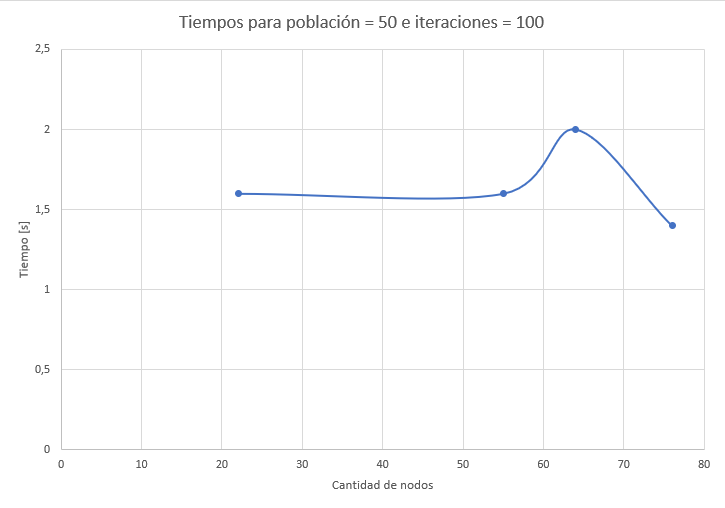
\includegraphics[width=1\textwidth]{Plantilla segundo entregable/graph1.png}
\caption{Tiempo vs cantidad de nodos para población de 50 individuos y 100 iteraciones.}
\end{figure} \\

Como se puede ver, no se logra apreciar alguna tendencia en el tiempo que le toma al algoritmo en terminar su ejecución, por lo que será mejor analizar el otro extremo que es con 100 individuos y 10000 iteraciones.

\begin{figure}[H]
\centering
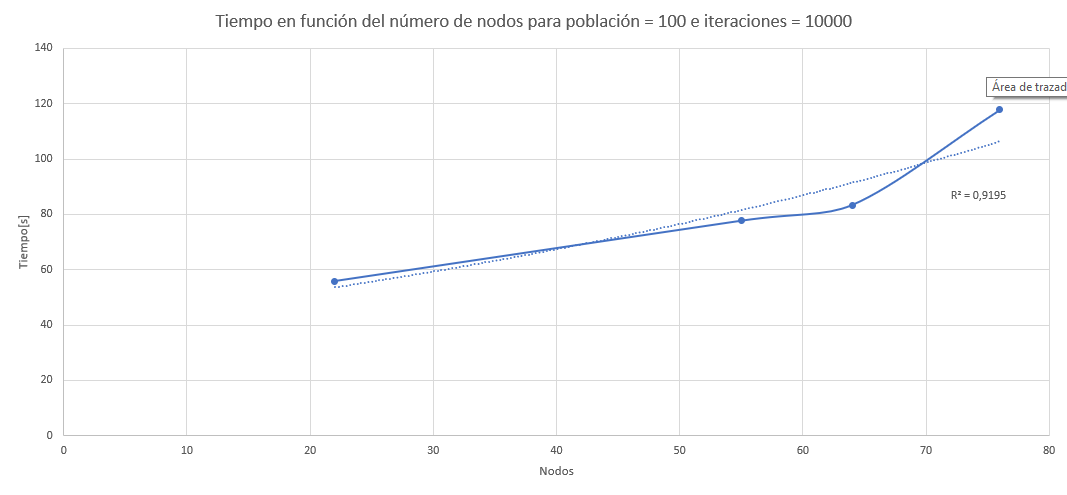
\includegraphics[width=1\textwidth]{Plantilla segundo entregable/graph3.png}
\caption{Tiempo vs cantidad de nodos para población de 100 individuos y 10000 iteraciones.}
\end{figure} \\

En este gráfico se realizó la línea de tendencia ajustando una curva exponencial. Como se puede apreciar, el valor de $R^2$ es relativamente alto, por lo que se podría decir que el tiempo aumenta de manera exponencial al aumentar la cantidad de nodos del problema. No obstante, se puede ver que el tiempo tampoco escapa a valores muy altos, por lo que habría que analizar los resultados obtenidos con más iteraciones para ver si vale la pena aumentar en tanto el número de estas. \\

Por otra parte, también interesa ver cómo se comporta el tiempo vs la cantidad de iteraciones.

\begin{figure}[H]
\centering
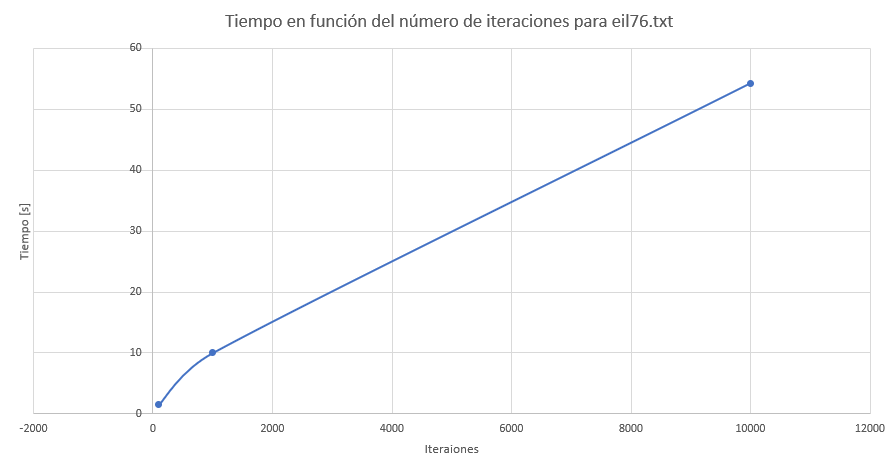
\includegraphics[width=1\textwidth]{Plantilla segundo entregable/graph2.png}
\caption{Tiempo vs cantidad de iteraciones para eil76.txt.}
\end{figure} \\

Como se esperaba, al aumentar el número de iteraciones (manteniendo el resto de cosas constante) el tiempo aumenta de manera relativamente lineal. \\

Otro dato interesante a analizar es las variaciones en las soluciones finales obtenidas en las iteraciones. En la figura siguiente se pueden apreciar los boxplot para todos los archivos.

\begin{figure}[H]
\begin{subfigure}{.5\textwidth}
  \centering
  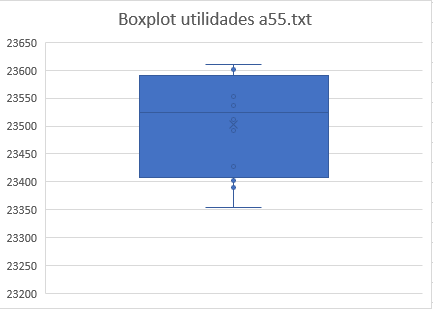
\includegraphics[width=.8\linewidth]{Plantilla segundo entregable/boxa55.png}
  \caption{Boxplot utilidades a55.txt.}
\end{subfigure}%
\begin{subfigure}{.5\textwidth}
  \centering
  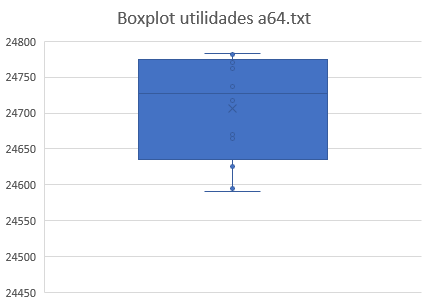
\includegraphics[width=.8\linewidth]{Plantilla segundo entregable/boxa64.png}
  \caption{Boxplot utilidades a64.txt.}
\end{subfigure}
\begin{subfigure}{.5\textwidth}
  \centering
  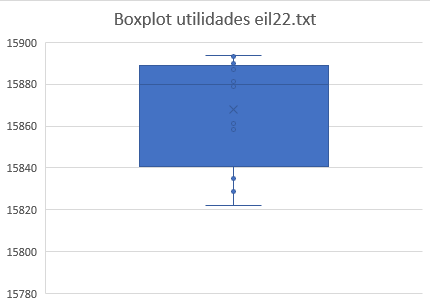
\includegraphics[width=.8\linewidth]{Plantilla segundo entregable/boxeil22.png}
  \caption{Boxplot utilidades eil22.txt.}
\end{subfigure}
\begin{subfigure}{.5\textwidth}
  \centering
  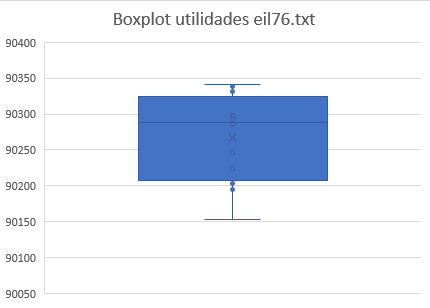
\includegraphics[width=.8\linewidth]{Plantilla segundo entregable/boxeil76.png}
  \caption{Boxplot utilidades eil76.txt.}
\end{subfigure}
\caption{Boxplot de las utilidades de cada instancia.}
\end{figure}

Dependiendo de la unidad estas diferencias pueden ser muy grandes o no. No obstante, los mayores valores se registran, en general, para los casos de 10000 iteraciones. Esto se puede deber a que, al darle al algoritmo más iteraciones (posibilidades de explorar y explotar al final) permite abarcar más lugar del espacio de soluciones y, por ende, terminar llegando a mejores soluciones que en los casos de menores iteraciones. 

\section{Conclusiones}

A lo largo de este semestre se ha investigado y desarrollado un algoritmo evolutivo para resolver el \textit{Milk Collection Problem with Blending}. Como el autor ha visto, desarrollar un algoritmo evolutivo no es tan simple como parece, menos cuando no se tiene un completo conocimiento del lenguaje de programación utilizado, por lo que este proyecto fue todo un desafío. Aunque no se logró resolver el problema para todas las instancias, las que sí se lograron resolver muestran la efectividad de las técnicas incompletas, obteniendo soluciones en cuestión de segundos incluso para instancias con diez mil iteraciones.\\

Se lograron confirmar cosas como que al aumentar la cantidad de variables (en este caso nodos) el tiempo de ejecución del algoritmo aumenta de manera exponencialmente, como también que la cantidad de iteraciones afecta de manera lineal al tiempo de ejecución. Por otra parte, no se logró apreciar una gran incidencia de un cambio de un 10\% en la probabilidad de cruzamiento, pero si una gran incidencia del número de iteraciones sobre el resultado final: al permitir que el algoritmo realice más iteraciones dejamos que este explore un mayor espacio de búsqueda y sea capaz de, en algunos casos, encontrar mejores soluciones que con menos iteraciones. \\

Sobre trabajo futuro, se sabe que las técnicas incompletas se ajustan a los parámetros y requisitos del problema, por lo que este algoritmo fue escrito pensado solamente para recibir tres camiones y tres tipos de leche, por lo que el siguiente paso es generar un algoritmo evolutivo genérico para poder resolver este problema con una cantidad variable de tipos de leches y camiones (el cual era el plan original, pero tuvo que ser cambiado en el trote). También, en general, analizar meta heurísticas que permitan el trabajo con genotipos con diferentes tamaños, ya que es una problemática que existe con soluciones no tan triviales.


%Secci\'on Referencias: Indicando toda la informaci\'on necesaria de acuerdo al tipo de documento revisado. Las referencias deben ser citadas en el documento.
\bibliographystyle{plain}
\bibliography{Referencias}
\end{document} 
